% =========================================================================
% 《高中數學實驗教材》第二冊（高一下） 
% 第一章 二次方程式
% =========================================================================

\section{二次方程式}\label{sec:b2_ch1}

在第一冊第四章中，我們會討論一次方程式及其應用\phantomsection\label{note:b2-ch1-intro-ceng}. 本章將繼續討論二次方程式及其應用. 引入未知數用方程式去解決問題的基本原理，並不因為方程式的次數不同而有所差別. 其實，對於一個實際的問題，其所對應的方程式的次數，究竟是多少，是要到我們列妥方程式並且加以整理後才能知道的. 一般說來，次數較高的方程式，其解法與討論也就比較困難.

\subsection{二次方程式——例子與解法}\label{sec:b2_1-1}

\subsubsection*{1-1 多項式的因子分解與方程式的解}

第一冊第五章中的餘式定理說：「$a$ 是 $f(x)=0$ 的一個根的必要充分條件是 $x-a$ 可以整除 $f(x)$，亦即 $x-a$ 是 $f(x)$ 式一個因子.」下述簡單事實更進一步地顯示「解方程式」和「多項式的因子分解」間所具有的密切關連.

\paragraph{方程式化簡原理：} 方程式 $g(x) \cdot h(x)=0$ 的解可以歸於方程式 $g(x)=0$ 及 $h(x)=0$ 的解. 換言之，方程式 $g(x)\cdot h(x)=0$ 的根也就是 $g(x)=0$ 的根或 $h(x)=0$ 的根. 所以我們只要分別去求出 $g(x)=0$ 的根以及 $h(x)=0$ 的根合起來也就是 $g(x)\cdot h(x)=0$ 的所有的根.

\noindent\textbf{【證明】}
$a$ 是 $g(x)\cdot h(x)=0$ 的根，
\begin{align*}
&\iff g(a)\cdot h(a)=0, \\
&\iff g(a)=0 \text{ 或 } h(a)=0, \\
&\iff \text{「$a$ 是 $g(x)=0$ 的根」或「$a$ 是 $h(x)=0$ 的根」.}
\end{align*}


依此類推，當 $f(x)$ 可以分解成其因子 $g_1(x), g_2(x), \dots, g_k(x)$ 的乘積時，亦即
\[
f(x)=g_1(x)\cdot g_2(x)\dotsm g_k(x),
\]
則解方程式 $f(x)=0$ 可以歸於解下列 $k$ 個方程式.
\[
g_1(x)=0,\ g_2(x)=0, \dots, g_k(x)=0
\]

\begin{example}\label{ex:b2_1-1-1}
解方程式 $x^2-5x+6=0$.
\end{example}
因為 $x^2-5x+6=(x-2)(x-3)$，
由於 $x^2-5x+6=0$ 的根也就是 $x-2=0$ 或 $x-3=0$ 的根，所以 $2$ 和 $3$ 都是 $x^2-5x+6=0$ 的根.

\begin{example}\label{ex:b2_1-1-2}
求 $x(x-1)(x-2)\dotsm(x-(k-1))(x-k)=0$ 的根.
\end{example}
求以上方程式的根可以先分別求以下諸方程式的根：
\[
x=0,\ x-1=0,\ x-2=0,\dots,x-k=0.
\]
所以原方程式的根為 $0, 1, 2, \dots, k$.

\begin{example}\label{ex:b2_1-1-3}
設 $g(x)=x(x+1)$，$h(x)=(x-3)(x+1)$. 問 $g(x)\cdot h(x)=0$ 有那些根？
\end{example}
$x(x+1)=0$ 的根為 $x=0$ 和 $x=-1$，\\
$(x-3)(x+1)=0$ 的根為 $x=3$ 和 $x=-1$.\\
\[
g(x)\cdot h(x)=x(x+1)^2(x-3)
\]
故 $g(x)\cdot h(x)=0$ 的根為 $x=0, -1, 3$.

在例三中\phantomsection\label{note:b2-ch1-ex3}，因為 $g(x)\cdot h(x)$ 有 $(x+1)^2$ 因子，我們說 $-1$ 是 $g(x)\cdot h(x)=0$ 的二重根，有時我們將重根重覆寫出. 例如 $g(x)\cdot h(x)=0$ 的根寫為 $0, -1, -1, 3$.

\subsubsection*{1-2 二次多項式的因子分解與二次方程式的解}

當一個二次多項式 $f(x)=a_2 x^2 + a_1 x + a_0$ 可以分解成兩個一次因子的乘積時，亦即
\[
f(x)=a_2 x^2 + a_1 x + a_0 = (b_1 x + b_0)(c_1 x + c_0),
\]
則方程式
\[
a_2 x^2 + a_1 x + a_0 = 0
\]
的解可歸於解下列兩個一次方程式：
\[
b_1 x + b_0 = 0, \text{ 以及 } c_1 x + c_0 = 0.
\]
所以 $b_1 x + b_0 = 0$ 的根 $-\frac{b_0}{b_1}$ 及 $c_1 x + c_0 = 0$ 的根 $-\frac{c_0}{c_1}$（註：$b_1, c_1$ 都不等於 $0$，因為 $b_1 c_1 = a_2 \ne 0$.）也就是 $f(x)=a_2 x^2 + a_1 x + a_0 = 0$ 的根. 反之當 $\alpha, \beta$ 是 $f(x)=0$ 的根時，由餘式定理可得
\[
f(x)=a_2(x-\alpha)(x-\beta).
\]
所以「解一個二次方程式 $a_2 x^2 + a_1 x + a_0 = 0$」和「把二次多項式 $a_2 x^2 + a_1 x + a_0$ 分解成二個一次因子的乘積」是一回事.

\begin{example}\label{ex:b2_1-1-4}
正方形的面積為 $144$ 平方公尺，問其邊長為幾公尺？
\end{example}
\noindent\textbf{【解】}
設其邊長為 $x$ 公尺，則其面積為 $x^2$ 平方公尺，即
\[
x^2 = 144 = 12^2
\]
顯然 $x = \pm 12$ 滿足上述方程式，但二次方程式最多只有兩個根，故上述方程式的解是 $x=12$ 及 $x=-12$，又依題意，$x$ 應為正值，故上述問題的答案是邊長為 $12$ 公尺.


\begin{example}\label{ex:b2_1-1-5}
設有一正方形，若其每邊加長 $6$ 公尺，則其面積是 $169$ 平方公尺，問其原邊長為幾公尺？
\end{example}
\noindent\textbf{【解】}
設其原邊長為 $x$ 公尺，則按題意有下列方程式
\[
(x+6)^2 = 169 = 13^2
\]
同學們不難看出 $x+6$ 應該等於 $\pm 13$，亦即 $x=\pm 13-6$，故 $7$ 及 $-19$ 是上述方程式的兩個根. 和例4一樣，對於上述問題，我們依題意只取其正根 $x=7$，即原邊長為 $7$ 公尺. 看起來似乎太簡單了，其實一般二次方程式的解法，也就是設法將一個要解的二次方程式，化簡為上述形式，亦即 $(x+b)^2=a^2$. 譬如：


\begin{example}\label{ex:b2_1-1-6}
有兵若干，列為方陣. 假若把他們改排成四列的中空方陣，則其外側一邊的人數較原方陣一邊的人數多 $16$ 人. 問有兵多少人？
\end{example}
\noindent\textbf{【解】}
設原方陣為每邊 $x$ 人，則共有兵 $x^2$ 人，\\
又外側每邊 $x+16$ 人的四列中空方陣共需
\[
(x+16)^2 - (x+8)^2 \text{ 人}.
\]
故有方程式
\begin{align*}
x^2 &= (x+16)^2 - (x+8)^2 \\
&= (x^2 + 32x + 16^2) - (x^2 + 16x + 8^2) \\
&= 16x + (256-64) \\
&= 16x + 192.
\end{align*}
亦即 $x^2-16x-192=0$.\\
利用配方法（將在 \S 2 中說明），上述又可以改寫為\phantomsection\label{note:b2-ch1-ex6}
\[
x^2 - 16x + 64 - 256 = 0,
\]
亦即 $(x-8)^2 = 16^2$.\\
故 $x-8 = \pm 16$,\\
即 $x=24$ 或 $x=-8$.\\
依題意只取其正值 $x=24$，故共有兵 $24^2 = 576$ 人.


\begin{figure}[htbp]
\centering
\begin{tikzpicture}[scale=0.85, >=latex]
  % 原方陣 (實心方陣)
  \draw[thick] (0, 3.2) rectangle (2.4, 5.6);
  \draw[<->] (0, 5.8) -- (2.4, 5.8) node[midway, above] {$x\text{ 人}$};

  % 四列中空方陣
  % 外側
  \draw[thick] (-0.8, -1.8) rectangle (3.2, 2.2);
  \draw[<->] (-0.8, 2.4) -- (3.2, 2.4) node[midway, above] {$x+16\text{ 人}$};
  % 內側
  \draw[thick] (0.2, -0.8) rectangle (2.2, 1.2);
  \draw[<->] (0.2, 1.4) -- (2.2, 1.4) node[midway, above] {$x+8\text{ 人}$};
\end{tikzpicture}
\caption{實心方陣與中空方陣示意圖}
\label{fig:soldier_formation}
\end{figure}

\begin{example}\label{ex:b2_1-1-7}
求方程式 $x^2+3x-18=0$ 的根.
\end{example}
\noindent\textbf{【解】}
因為 $(x+\frac{3}{2})^2 = x^2+3x+\frac{9}{4}$.\\
故有 $x^2+3x-18 = (x+\frac{3}{2})^2 - (18+\frac{9}{4}) = 0$\\
亦即
\[
\left(x+\frac{3}{2}\right)^2 = \frac{81}{4} = \left(\frac{9}{2}\right)^2
\]
故
\[
x = \pm \frac{9}{2} - \frac{3}{2} = -\frac{12}{2},\ \frac{6}{2},
\]
亦即 $x = -6,\ 3.$


\begin{example}\label{ex:b2_1-1-8}
解 $6x^2+x-15=0$.
\end{example}
\noindent\textbf{【解】}
原式可寫為 $x^2+\frac{1}{6}x-\frac{15}{6}=0$\\
因為
\[
x^2+\frac{1}{6}x-\frac{15}{6} = \left(x+\frac{1}{12}\right)^2 - \left(\frac{15}{6}+\frac{1}{144}\right) = 0.
\]
亦即
\[
\left(x+\frac{1}{12}\right)^2 = \frac{361}{144} = \left(\frac{19}{12}\right)^2
\]
開方得
\[
x+\frac{1}{12} = \pm \frac{19}{12}.
\]
即得 $x = \frac{3}{2},\ -\frac{5}{3}.$


以上用配方法解二次方程式固然適合於各種情形，但有時卻以另一種方法來解更為簡便，我們先分析如下：

設 $a_2 x^2 + a_1 x + a_0 = 0$ 為我們要解的方程式. 而
\begin{equation}\label{eq:b2_factor_rel}
a_2 x^2 + a_1 x + a_0 = (b_1 x + b_0)(c_1 x + c_0) \dots\dots\dots (1)
\end{equation}
那麼，我們知道 $x = -\frac{b_0}{b_1}$ 和 $-\frac{c_0}{c_1}$，故我們先來討論此二次式係數與其一次因式係數的關係. 將 \eqref{eq:b2_factor_rel} 右邊乘開可得 $b_1 c_1 x^2 + (b_1 c_0 + b_0 c_1)x + b_0 c_0$. 所以比較兩邊係數後，可以看出
\begin{align*}
a_2 &= b_1 c_1, \\
a_1 &= b_1 c_0 + b_0 c_1, \\
a_0 &= b_0 c_0.
\end{align*}
由以上討論可得另一解法，稱為交叉因子分解法；分下述四個步驟：
\begin{enumerate}[(一)]
  \item 將 $a_2, a_0$ 分別寫為任意兩個因數的乘積.
  \begin{align*}
  a_2 &= {b_1}' {c_1}', \\
  a_0 &= {b_0}' {c_0}'.
  \end{align*}
  \item 寫成
  \begin{center}
  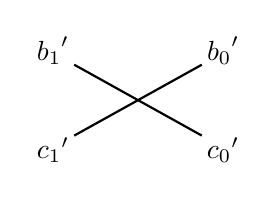
\begin{tikzpicture}[scale=0.9, baseline=(current bounding box.center)]
    \node at (0, 1.2) {${b_1}'$};
    \node at (2.4, 1.2) {${b_0}'$};
    \node at (0, -0.2) {${c_1}'$};
    \node at (2.4, -0.2) {${c_0}'$};
    \draw[thick] (0.3, 1.0) -- (2.1, 0.0);
    \draw[thick] (0.3, 0.0) -- (2.1, 1.0);
  \end{tikzpicture}
  \end{center}
  並交叉相乘，得 ${b_1}' {c_0}'$ 和 ${b_0}' {c_1}'$.
  \item 驗證是否 ${b_1}' {c_0}' + {b_0}' {c_1}' = a_1$. 如果是的話，則原二次式可寫為 $({b_1}' x + {b_0}')({c_1}' x + {c_0}')$，而其根也就求出來了.
  \item 如果不是的話，以別的因數的積再試.
\end{enumerate}

以上方法對於根為整數時，才較為簡便，我們把上面的【例7】，【例8】用此法再做一遍：

\paragraph{【例7】} $x^2 + 3x - 18 = 0$.
\[
-18 = 6 \cdot (-3).
\]
\begin{center}
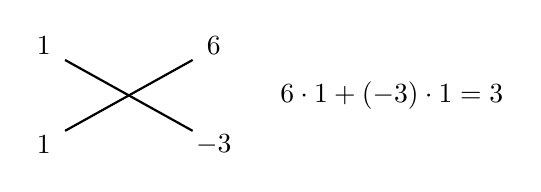
\begin{tikzpicture}[scale=0.9, baseline=(current bounding box.center)]
  \node at (0, 1.2) {$1$};
  \node at (2.4, 1.2) {$6$};
  \node at (0, -0.2) {$1$};
  \node at (2.4, -0.2) {$-3$};
  \draw[thick] (0.3, 1.0) -- (2.1, 0.0);
  \draw[thick] (0.3, 0.0) -- (2.1, 1.0);
  \node[anchor=west] at (3.2, 0.5) {$6 \cdot 1 + (-3) \cdot 1 = 3$};
\end{tikzpicture}
\end{center}
\[
(x+6)(x-3) = 0. \qquad \therefore\ x = -6,\ 3.
\]

\paragraph{【例8】} $6x^2 + x - 15 = 0$.
\begin{align*}
6 &= 3 \cdot 2, \\
-15 &= 5 \cdot (-3).
\end{align*}
\begin{center}
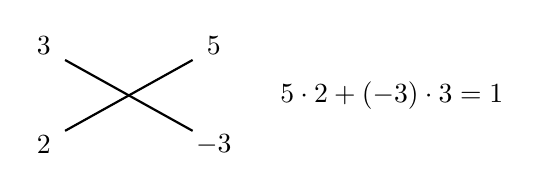
\begin{tikzpicture}[scale=0.9, baseline=(current bounding box.center)]
  \node at (0, 1.2) {$3$};
  \node at (2.4, 1.2) {$5$};
  \node at (0, -0.2) {$2$};
  \node at (2.4, -0.2) {$-3$};
  \draw[thick] (0.3, 1.0) -- (2.1, 0.0);
  \draw[thick] (0.3, 0.0) -- (2.1, 1.0);
  \node[anchor=west] at (3.2, 0.5) {$5 \cdot 2 + (-3) \cdot 3 = 1$};
\end{tikzpicture}
\end{center}
\[
(3x+5)(2x-3) = 0. \qquad \therefore\ x = -\frac{5}{3},\ \frac{3}{2}.
\]

\subsubsection*{習題 1-1}\label{sec:b2_ex1-1}

\begin{enumerate}
  \item 解下列各方程式：
  \begin{enumerate}[(i)]
    \item $x^2-3x+1=0$.
    \item $x^2+5x-4=0$.
    \item $x^2+20x+64=0$.
    \item $(x^2-6x+2)(x-1)(x+2)=0$.
    \item $(x^2+3x+1)(x^2-3x+1)=0$.
    \item $(x+5)^2=4x+20$.
    \item $x^4-25x^2+144=0$.
    \item $6x^4-5x^2+1=0$.
    \item $(2x^2-x)^2 - 4(2x^2-x) + 3 = 0$.
    \item $(2x^2-5x)^2+4x=10x+3$.
    \item $x-8\sqrt{x}+15=0$.
    \item $\sqrt{x}-29=-\dfrac{30}{\sqrt{x}}$.
  \end{enumerate}

  \item 用交叉因子分解法，解下列各方程式：
  \begin{enumerate}[(i)]
    \item $6x^2+x-2=0$.
    \item $20x^2-13x+2=0$.
    \item $21x^2+13x+2=0$.
    \item $20x^2-3x-9=0$.
  \end{enumerate}

  \item 把石頭用 $16.8$（公尺/秒）的初速度拋上去，那麼高度 $S$（公尺）是時間 $t$（秒）的二次函數. $S=-490t^2+16.8t$\phantomsection\label{note:b2-ch1-gravity}，問什麼時候高度是 $14$ 公尺？

  \item 若將一立方體的各邊長增加 $2$ 公分，則其體積增加 $386$ 立方公分，求原來立方體的邊長.
\end{enumerate}

\subsection{配方與公式解}\label{sec:b2_1-2}

現在讓我們來討論一般解二次方程式的方法. 設方程式為
\begin{equation}\label{eq:b2_quad_standard}
ax^2+bx+c=0,\ a \ne 0 \dots\dots\dots\dots\dots\dots\dots (1)
\end{equation}
首先，我們可以將上式各項除以 $a$，而得下列首項係數為 $1$ 的式子：
\begin{equation}\label{eq:b2_quad_div_a}
x^2+\frac{b}{a}x+\frac{c}{a}=0 \dots\dots\dots\dots\dots\dots\dots (2)
\end{equation}
又因
\begin{equation}\label{eq:b2_complete_square_id}
\left(x+\frac{b}{2a}\right)^2=x^2+\frac{b}{a}x+\left(\frac{b}{2a}\right)^2 \dots\dots\dots\dots\dots\dots\dots (3)
\end{equation}
故(2)式可以重寫為
\[
\left(x+\frac{b}{2a}\right)^2 = \left(\frac{b}{2a}\right)^2 - \frac{c}{a} = \frac{b^2-4ac}{4a^2}.
\]
即得
\[
x+\frac{b}{2a} = \pm \sqrt{\frac{b^2-4ac}{4a^2}} = \frac{\pm \sqrt{b^2-4ac}}{2a}.
\]
亦即
\begin{equation}\label{eq:b2_quad_sol}
x = -\frac{b}{2a} \pm \frac{\sqrt{b^2-4ac}}{2a} = \frac{-b \pm \sqrt{b^2-4ac}}{2a} \dots\dots (4)
\end{equation}

\paragraph{注意：}
\begin{enumerate}[(i)]
  \item 當 $b^2-4ac$ 是負數時，則 $\sqrt{b^2-4ac}$ 顯然不可能是一個實數，因為任何實數的平方總是 $\ge 0$. 在這種情形下，我們叫 $\sqrt{b^2-4ac}$ 為一虛數. 其意義將在以後再詳加闡述.
  \item 有些書在一開始就把 (1) 式寫成 $ax^2+2bx+c=0$，採用這樣的符號，則顯然有公式
  \[
  x = \frac{-b \pm \sqrt{b^2-ac}}{a}
  \]
  （以 $2b$ 代替 $b$，代入 (4) 式化簡即得）.
\end{enumerate}

我們把上述討論的結論，敘述為下列定理：

\begin{theorem}\label{thm:b2_1-1}
方程式
\[
ax^2+bx+c=0,\quad a \ne 0
\]
的根可以由下述公式求得：
\begin{equation}\label{eq:b2_quad_formula_thm}
x = \frac{-b \pm \sqrt{b^2-4ac}}{2a} \dots\dots\dots\dots\dots\dots\dots (4)
\end{equation}
\end{theorem}

\paragraph{注意：} 在求得上述公式的過程中，最要緊的是把 $x^2+\frac{b}{a}x$ 改寫成 $(x+\frac{b}{2a})^2 - \frac{b^2}{4a^2}$，即
\begin{equation}\label{eq:b2_completing_square_thm}
x^2+\frac{b}{a}x = \left(x+\frac{b}{2a}\right)^2 - \left(\frac{b}{2a}\right)^2 \dots\dots\dots\dots\dots\dots\dots (5)
\end{equation}
這種步驟叫做配方，它在二次式的討論中是很重要的.

\begin{corollary}\label{cor:b2_1-1}
任意二次多項式 $ax^2+bx+c$，在形式上都可以作下列因子分解，即
\[
ax^2+bx+c = a\left(x - \frac{-b+\sqrt{b^2-4ac}}{2a}\right)\left(x - \frac{-b-\sqrt{b^2-4ac}}{2a}\right).
\]
\end{corollary}

\begin{corollary}\label{cor:b2_1-2}
任意二元二次齊次式 $ax^2+bxy+cy^2$，在形式上都可以作下列因式分解. 即
\[
ax^2+bxy+cy^2 = a\left(x - \frac{-b+\sqrt{b^2-4ac}}{2a}y\right)\left(x - \frac{-b-\sqrt{b^2-4ac}}{2a}y\right).
\]
\hfill （證明留做習題）\phantomsection\label{note:b2-ch1-cor2}
\end{corollary}

\subsubsection*{習題 1-2}\label{sec:b2_ex1-2}

\begin{enumerate}
  \item 試證上面的推論 2.

  \item 用公式解下列方程式：
  \begin{enumerate}[(i)]
    \item $x^2+2x-1=0$.
    \item $x^2+x+1=0$.
    \item $(\sqrt{5}-2)x^2-2x+4=0$.
    \item $(x+2)(x+3)(x-4)=x^3$.
    \item $2x^2+3x=4$.
  \end{enumerate}

  \item 分解下列二次齊次式為一次因式：
  \begin{enumerate}[(i)]
    \item $3x^2-10xy+3y^2$.
    \item $x^2+xy+y^2$.
    \item $a^2-4ab+2b^2$.
    \item $2a^2-2ab-b^2$.
  \end{enumerate}
\end{enumerate}

\subsection{根與係數的關係、判別式與二次方程式的討論}\label{sec:b2_1-3}

\subsubsection*{3-1 本節符號用法}

在這一節裡，我們將依然用 $ax^2+bx+c=0$ 表示一個一般的二次方程式. 我們將用 $\alpha, \beta$ 表示它的根，以 $\delta$ 表示 $b^2-4ac$. 即
\[
\delta = b^2-4ac,
\]
這式叫做該方程式的判別式.

\subsubsection*{3-2 根與係數的關係}

設 $\alpha, \beta$ 為 $ax^2+bx+c=0$ 的根，則由餘式定理得
\begin{align*}
ax^2+bx+c &= a\cdot \left(x^2+\frac{b}{a}x+\frac{c}{a}\right) \\
&= a\cdot (x-\alpha)(x-\beta) \\
&= a\cdot [x^2-(\alpha+\beta)x+\alpha\beta].
\end{align*}
依多項式相等的定義，上面左右兩邊各項係數應該相等. 故有下述根與係數關係：
\[
\alpha+\beta = -\frac{b}{a},
\]
\[
\alpha\beta = \frac{c}{a}.
\]

\begin{example}\label{ex:b2_1-3-1}
設 $\alpha, \beta$ 為二次方程式 $2x^2+3x+6=0$ 的兩根，則有
\begin{align*}
\alpha+\beta &= -\frac{3}{2}, \\
\alpha\beta &= 3.
\end{align*}
\end{example}

\begin{example}\label{ex:b2_1-3-2}
求以 $\dfrac{p-q}{p+q}$ 與 $\dfrac{-(p+q)}{p-q}$ 為兩根的二次方程式.
\end{example}
\noindent\textbf{【解】}
設兩根為 $\alpha$ 與 $\beta$，則
\begin{align*}
\alpha+\beta &= \frac{p-q}{p+q} - \frac{p+q}{p-q} = \frac{(p-q)^2 - (p+q)^2}{p^2-q^2} \\
&= \frac{-4pq}{p^2-q^2}, \\
\alpha\beta &= \frac{p-q}{p+q} \cdot \left(-\frac{p+q}{p-q}\right) = -1.
\end{align*}
所以
\[
x^2 + \frac{4pq}{p^2-q^2}x - 1 = 0 \text{ 以 } \alpha, \beta \text{ 為根}.
\]
\[
\therefore \quad (p^2-q^2)x^2 + 4pqx - (p^2-q^2) = 0
\]
為我們所求的一個方程式.


\begin{example}\label{ex:b2_1-3-3}
設 $ax^2+bx+c=0$ 的兩根之比為 $m:n$，試證
\[
mnb^2 = (m+n)^2 ac.
\]
\end{example}
\noindent\textbf{【解】}
設兩根為 $m\alpha, n\alpha$. 由根與係數的關係得
\begin{align}
(m+n)\alpha &= -\frac{b}{a} \dots\dots\dots\dots\dots\dots\dots\dots\dots\dots (1) \label{eq:b2_root_ratio_sum} \\
mn\alpha^2 &= \frac{c}{a} \dots\dots\dots\dots\dots\dots\dots\dots\dots\dots (2) \label{eq:b2_root_ratio_prod}
\end{align}
由 \eqref{eq:b2_root_ratio_sum} 得 $\alpha = \dfrac{-b}{(m+n)a}$，代入 \eqref{eq:b2_root_ratio_prod} 式得
\[
mn\left[\frac{-b}{a(m+n)}\right]^2 = \frac{c}{a}
\]
通分得 $mnb^2 = (m+n)^2 ac$，故得證.


\subsubsection*{3-3 二次方程式的討論}

在上節公式 (4) $x = \dfrac{-b \pm \sqrt{b^2-4ac}}{2a}$ 可知兩根相等的充分必要條件是 $\delta = b^2-4ac = 0$. 而當 $\delta > 0$ 時，$ax^2+bx+c=0$ 有相異的二實根，當 $\delta < 0$ 時，其根為 $\dfrac{-b \pm \sqrt{b^2-4ac}}{2a}$ 的形式，其中 $\sqrt{b^2-4ac}$ 為一虛數. 習慣上，這種根叫做虛根.

綜合上述討論，可敘述為下列定理.

\begin{theorem}\label{thm:b2_1-2}
對於二次方程式 $ax^2+bx+c=0$，$a \ne 0$. 根與係數間有下列關係：
\begin{enumerate}[(i)]
  \item 二根之和為 $-\frac{b}{a}$，二根之積為 $\frac{c}{a}$（即 $\alpha+\beta = -\frac{b}{a}$，$\alpha\beta = \frac{c}{a}$）.
  \item
  \[
  \begin{cases}
  \delta = 0 \iff \text{有二相等實根（亦稱為二重根）}. \\
  \delta > 0 \iff \text{有二相異實根}. \\
  \delta < 0 \iff \text{有二相異虛根}.
  \end{cases}
  \]
\end{enumerate}
\end{theorem}

\begin{example}\label{ex:b2_1-3-4}
設 $x^2+8x+q=0$ 的二根之差的平方為 $4$，求 $q$ 的值.
\end{example}
\noindent\textbf{【解】}
令 $\alpha, \beta$ 為上述方程式的二根，則由假設得
\[
(\alpha-\beta)^2 = 4.
\]
但是由等式 $(\alpha-\beta)^2 = \alpha^2-2\alpha\beta+\beta^2 = (\alpha^2+2\alpha\beta+\beta^2)-4\alpha\beta = (\alpha+\beta)^2-4\alpha\beta$，故由根與係數的關係即得
\[
4 = 8^2-4q = 64-4q,\qquad q=15.
\]


\begin{example}\label{ex:b2_1-3-5}
設 $x^2+px+q=0$ 的二根為 $\alpha, \beta$. 求以 $\alpha^2+\beta$ 和 $\beta^2+\alpha$ 為根的二次方程式.
\end{example}
\noindent\textbf{【解】}
設所求的方程式為 $x^2+bx+c=0$，則根與係數的關係為
\[
\begin{cases}
(\alpha^2+\beta)+(\beta^2+\alpha) = -b \\
(\alpha^2+\beta)\cdot(\beta^2+\alpha) = c
\end{cases}, \qquad
\begin{cases}
\alpha+\beta = -p \\
\alpha\beta = q
\end{cases}.
\]
我們得把 $b, c$ 用原方程式的係數 $p, q$ 表出. 換言之，我們得設法把 $\alpha^2+\beta^2+\alpha+\beta$ 和 $\alpha^2\beta^2+\alpha\beta+\alpha^3+\beta^3$ 用 $\alpha+\beta$ 和 $\alpha\beta$ 表出，同學們不難由展開得下述等式：
\begin{align*}
(\alpha+\beta)^2 &= \alpha^2+2\alpha\beta+\beta^2; \\
\text{即}\qquad \alpha^2+\beta^2 &= (\alpha+\beta)^2-2\alpha\beta. \\
(\alpha+\beta)^3 &= \alpha^3+3\alpha^2\beta+3\alpha\beta^2+\beta^3, \\
\text{即}\qquad \alpha^3+\beta^3 &= (\alpha+\beta)^3-3\alpha\beta\cdot(\alpha+\beta).
\end{align*}
故有
\begin{align*}
-b &= (\alpha^2+\beta^2)+(\alpha+\beta) = (\alpha+\beta)^2-2\alpha\beta+(\alpha+\beta) \\
&= p^2-p-2q. \\
c &= \alpha^2\beta^2+\alpha\beta+(\alpha^3+\beta^3) = (\alpha\beta)^2+\alpha\beta+(\alpha+\beta)^3 - 3\alpha\beta(\alpha+\beta) \\
&= q^2+q+3qp-p^3.
\end{align*}
亦即所求方程式為
\[
x^2-(p^2-p-2q)x + (q^2+q+3qp-p^3) = 0.
\]


\subsubsection*{習題 1-3}\label{sec:b2_ex1-3}

\begin{enumerate}
  \item 找一個整係數二次方程式，使它的根是：
  \begin{enumerate}[(i)]
    \item $-3, 8$.
    \item $\dfrac{1}{2}, -\dfrac{5}{3}$.
    \item $-1+\sqrt{2}, -1-\sqrt{2}$.
    \item $-2+\sqrt{3}, -2-\sqrt{3}$.
  \end{enumerate}

  \item 甲，乙兩人解同一個二次方程式，甲將第二項 $x$ 的係數看錯，解得二根為 $-3, -4$；乙將第三項常數看錯，解得二根為 $2, 5$；你的答案是多少？

  \item 如果 $ax^2+bx+c=0$ 的兩根是 $\alpha, \beta$，找一個二次方程式，使它的根是：
  \begin{enumerate}[(i)]
    \item $2\alpha, 2\beta$.
    \item $\alpha+1, \beta+1$.
    \item $\alpha^2, \beta^2$.
    \item $\dfrac{1}{\alpha}, \dfrac{1}{\beta}$.
  \end{enumerate}

  \item 如果 $ax^2+bx+c=0$ 的根是 $\alpha, \beta$，請用 $a, b, c$ 表示
  \begin{enumerate}[(i)]
    \item $\dfrac{1}{\alpha} + \dfrac{1}{\beta}$.
    \item $(\alpha-1)(\beta-1)$.
    \item $\dfrac{\beta}{\alpha} + \dfrac{\alpha}{\beta}$.
    \item $\alpha^3 + \beta^3$.
  \end{enumerate}

  \item 試證 $(a+b)x^2 - (a+b+c)x + \dfrac{c}{2} = 0$ 有實根.
\end{enumerate}

\subsection{應用}\label{sec:b2_1-4}

\subsubsection*{4-1 二次函數的極大、極小}

在第一冊第五章中我們說過：任何一個多項式 $f(x)$，都有一個對應的多項式函數 $y=f(x)$；因此對於一個二次多項式 $ax^2+bx+c$，我們有一個對應的二次函數
\begin{equation}\label{eq:b2_quad_func}
y = ax^2+bx+c \dots\dots\dots\dots\dots\dots\dots\dots\dots\dots (1)
\end{equation}
由 \S 2 配方的計算，我們可以把(1)式重寫為
\begin{align}
y &= a\left[\left(x+\frac{b}{2a}\right)^2 + \frac{4ac-b^2}{4a^2}\right] \nonumber \\
&= a\left[\left(x+\frac{b}{2a}\right)^2 + \frac{(-\delta)}{4a^2}\right] \dots\dots\dots\dots\dots\dots\dots (2) \label{eq:b2_quad_vertex}
\end{align}
顯然，當 $x$ 為任何實數時，均有
\begin{equation}\label{eq:b2_square_nonneg}
\left(x+\frac{b}{2a}\right)^2 \ge 0, \text{（``$=$''僅在 $x=-\frac{b}{2a}$ 時成立）} \dots\dots (3)
\end{equation}
故有
\[
\left(x+\frac{b}{2a}\right)^2 + \frac{-\delta}{4a^2} \ge \frac{-\delta}{4a^2}, \text{（``$=$''僅於 $x=-\frac{b}{2a}$ 時成立）}
\]
所以當 $a > 0$ 時，我們有
\[
y = a\cdot \left[\left(x+\frac{b}{2a}\right)^2 + \frac{-\delta}{4a^2}\right] \ge \frac{-\delta}{4a^2}\cdot a = \frac{-\delta}{4a} = f\left(-\frac{b}{2a}\right).
\]
亦即當 $a>0$ 時，二次函數 $y=ax^2+bx+c$ 在 $x=-\frac{b}{2a}$ 時的函數值
\[
f\left(-\frac{b}{2a}\right) = \frac{-\delta}{4a} = \frac{4ac-b^2}{4a}
\]
是該函數的極小值. 反之，當 $a<0$ 時，我們有
\[
y = a\cdot \left[\left(x+\frac{b}{2a}\right)^2 + \frac{-\delta}{4a^2}\right] \le \frac{-\delta}{4a^2}\cdot a = \frac{-\delta}{4a} = f\left(-\frac{b}{2a}\right).
\]
亦即當 $a<0$ 時，二次函數 $y=ax^2+bx+c$ 在 $x=-\frac{b}{2a}$ 時的函數值 $f\left(-\frac{b}{2a}\right) = \frac{-\delta}{4a}$ 是它的極大值.

\begin{theorem}\label{thm:b2_1-3}
二次函數 $y=ax^2+bx+c$ 在 $x=-\frac{b}{2a}$ 時的函數值
\[
f\left(-\frac{b}{2a}\right) = \frac{-\delta}{4a} = \frac{4ac-b^2}{4a}
\]
不是極大就是極小：當 $a<0$ 時為極大；$a>0$ 時為極小.
\end{theorem}

\begin{corollary}\label{cor:b2_1-3}
對於一個二次函數 $y=ax^2+bx+c$，
\begin{enumerate}[(i)]
  \item 其函數值永不為負（亦即 $f(x)$ 永遠 $\ge 0$）的充分必要條件是「$a>0$ 和 $\delta \le 0$」.
  \item 其函數值永不為正（亦即 $f(x)$ 永遠 $\le 0$）的充分必要條件是「$a<0$ 和 $\delta \le 0$」.
\end{enumerate}
\end{corollary}

\begin{example}\label{ex:b2_1-4-1}
今有一 $400$ 公尺長的鐵絲網一捲，用來圍一塊長方形的地，問最多可以圍多少平方公尺？
\end{example}
\noindent\textbf{【解】}
令 $x$ 為此長方形的寬，則 $\frac{1}{2}(400-2x) = 200-x$ 為其長，故長方形的面積為
\[
y = x\cdot (200-x) = -x^2+200x.
\]

\begin{figure}[htbp]
\centering
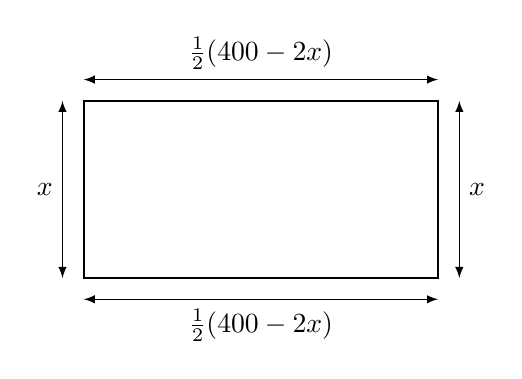
\begin{tikzpicture}[scale=0.9, >=latex]
  \draw[thick] (0, 0) rectangle (5, 2.5);
  % 寬度標註
  \draw[<->] (-0.3, 0) -- (-0.3, 2.5) node[midway, left] {$x$};
  \draw[<->] (5.3, 0) -- (5.3, 2.5) node[midway, right] {$x$};
  % 長度標註
  \draw[<->] (0, 2.8) -- (5, 2.8) node[midway, above] {$\frac{1}{2}(400-2x)$};
  \draw[<->] (0, -0.3) -- (5, -0.3) node[midway, below] {$\frac{1}{2}(400-2x)$};
\end{tikzpicture}
\caption{鐵絲網圍成長方形示意圖}
\label{fig:fenced_field}
\end{figure}

由定理3，當 $x = \frac{-b}{2a} = 100$ 時，上述函數得其極大值 $10000 = f(100)$，故當所圍者是一個 $100 \times 100$ 的正方形時，面積最大，共計 $10000$ 平方公尺.


\begin{example}\label{ex:b2_1-4-2}
今有一高射砲彈，它在出砲口時的「垂直分速」是 $400$ 公尺/秒.「水平分速」是 $100$ 公尺/秒. 若將空氣阻力略去不計時，試求它的「彈道」（註）的「最高點」的高度？它落地時和原砲位的水平距離？
\end{example}
\noindent\textbf{【解】}
對於上述物理問題，地心引力是影響該砲彈飛行的最主要因素.（其次要者如空氣阻力，氣流速度等均已略去不計.）它使砲彈在垂直方向產生 $-9.8$ 公尺/秒$^2$ 的加速度，故砲彈在垂直方向的投影是一個加速度為 $-9.8$ 公尺/秒$^2$ 的等加速運動，由等加速運動的距離公式有
\[
y = t\text{ 秒的高度} = \left(400\cdot t - \frac{1}{2}(9.8)\cdot t^2\right) \text{ 公尺}.
\]
由定理 3 得知，當 $t = \frac{-b}{2a}$ 秒時砲彈達最高點，其高度為
\[
f\left(-\frac{b}{2a}\right) = \frac{4ac-b^2}{4a} = \frac{(400)^2}{2\cdot(9.8)} = 8163\text{ 公尺}.
\]
即最高點的高度約為 $8163$ 公尺.

\begin{figure}[htbp]
\centering
\begin{tikzpicture}[scale=1.1, >=latex]
  % 坐標軸
  \draw[->, thick] (0, 0) -- (0, 5.5);
  \node[left] at (-0.05, 3.2) {\shortstack{高\\度}};
  \draw[->, thick] (0, 0) -- (6.5, 0);
  \node[below] at (3.2, -0.1) {水平距離};

  % 拋物線彈道
  \draw[very thick] (0, 0) parabola bend (2.8, 4.8) (5.6, 0);

  % 重力向下箭頭
  \draw[->, very thick] (2.8, 3.8) -- (2.8, 2.6);
  \node[below] at (2.8, 2.5) {\shortstack{重\\力}};
\end{tikzpicture}
\caption{拋射物體彈道示意圖}
\label{fig:trajectory}
\end{figure}

因水平方向的運動是不受地心引力的影響的，所以其水平投影是一個等速運動，即
\[
t\text{ 秒的水平距離} = (100\cdot t)\text{ 公尺}
\]
由 $y = 400t - \frac{1}{2}(9.8)\cdot t^2 = 0$ 可以求得其落地的時間為
\[
t = \frac{400}{4.9} = 81.63\text{ 秒}.
\]
故落地時的水平距離為
\[
100\cdot (81.63) = 8163 \text{ 公尺}.
\]


\begin{remark}
砲彈飛行所經過的軌跡，軍事術語叫做彈道，在數學中，這一類由拋擲物體所成的軌跡叫做拋物線，其種種性質將在以後再詳加討論.
\end{remark}

\begin{example}\label{ex:b2_1-4-3}
設 $a_1, a_2, a_3, b_1, b_2, b_3$ 為任意實數，則顯然下述函數值永不為負.
\end{example}
\noindent\textbf{【解】}
\begin{align*}
y &= (a_1 x+b_1)^2 + (a_2 x+b_2)^2 + (a_3 x+b_3)^2 \\
&= (a_1^2+a_2^2+a_3^2)x^2 + 2\cdot (a_1 b_1 + a_2 b_2 + a_3 b_3)x + (b_1^2+b_2^2+b_3^2) \ge 0.
\end{align*}
故由推論，即得
\[
\delta = 4\cdot (a_1 b_1 + a_2 b_2 + a_3 b_3)^2 - 4\cdot (a_1^2+a_2^2+a_3^2)(b_1^2+b_2^2+b_3^2) \le 0
\]
亦即
\[
(a_1 b_1 + a_2 b_2 + a_3 b_3)^2 \le (a_1^2+a_2^2+a_3^2)(b_1^2+b_2^2+b_3^2)
\]
上述不等式叫做舒瓦茲（Schwarz）不等式，它和幾何中的「三角形兩邊的和大于第三邊」具有密切關連. 以後我們還會對此詳加剖析的.


\subsubsection*{習題 1-4}\label{sec:b2_ex1-4}

\begin{enumerate}
  \item 求下列各方程式的極大或極小：
  \begin{enumerate}[(i)]
    \item $y = 2x^2-x+4$.
    \item $y = -5x^2-4x+2$.
    \item $y = x(x+1)$.
    \item $y = -x^2-3x+2$.
    \item $y = -7x^2+6x-1$.
  \end{enumerate}

  \item 求內接於圓而面積最大的矩形，和周界最大的矩形.

  \item 設線段 $\overline{AB}$ 的長是 $a$，在 $\overline{AB}$ 上任取一點 $P$，以線段 $\overline{AB}$ 和 $\overline{PB}$ 為一邊各作一正方形\phantomsection\label{note:b2-ch1-ex1-4-q3}. 如果要使這兩個正方形面積的和為最小，試求 $P$ 點的位置應該在那裏？

  \item 如下圖，$\overline{AB}$ 是一條長 $24$ 公分的鐵絲，$P$ 是 $\overline{AB}$ 上一點，將 $\overline{PB}$ 分為四等分，使它圍成一正方形 $PSTU$；將 $AP$ 分為三等分，使其實成一正三角形 $PQR$\phantomsection\label{note:b2-ch1-ex1-4-q4}. $R, U, P$ 三點決定一三角形，問 $P$ 在何處時 $\triangle UPR$ 面積最大.

  \begin{figure}[htbp]
  \centering
  \begin{tikzpicture}[scale=1.0, >=latex]
    % 基準線 AB
    \coordinate (A) at (-3, 0);
    \coordinate (Q) at (-1.5, 0);
    \coordinate (P) at (0, 0);
    \coordinate (S) at (1.5, 0);
    \coordinate (B) at (3, 0);

    \draw[thick] (A) -- (B);

    % 正三角形 PQR (邊長 QP = 1.5)
    \coordinate (R) at (-0.75, 1.299);
    \draw[thick] (Q) -- (R) -- (P);

    % 正方形 PSTU (邊長 PS = 1.5)
    \coordinate (T) at (1.5, 1.5);
    \coordinate (U) at (0, 1.5);
    \draw[thick] (P) -- (S) -- (T) -- (U) -- cycle;

    % 陰影三角形 UPR
    \fill[pattern=north east lines, pattern color=black!60] (U) -- (P) -- (R) -- cycle;
    \draw[thick] (U) -- (R);
    \draw[thick] (U) -- (P);
    \draw[thick] (P) -- (R);

    % 標籤
    \node[below] at (A) {$A$};
    \node[below] at (Q) {$Q$};
    \node[below] at (P) {$P$};
    \node[below] at (S) {$S$};
    \node[below] at (B) {$B$};

    \node[above] at (R) {$R$};
    \node[above] at (U) {$U$};
    \node[above] at (T) {$T$};

    % 端點大括號/標記
    \draw[thick] (-3, 0) ++(-0.1, 0.4) arc (120:240:0.25);
    \draw[thick] (3, 0) ++(0.1, -0.05) arc (-60:60:0.25);
  \end{tikzpicture}
  \caption{正三角形與正方形幾何配置圖}
  \label{fig:triangle_square}
  \end{figure}

  \item 設 $y$ 為 $x$ 之二次多項式，而當 $x=0, 1, 2$ 時，$y$ 分別為 $8, 5, 6$，試求 $y$.
\end{enumerate}

\subsubsection*{4-2 二次聯立方程式}

就如同解二元、三元一次聯立方程式，我們可以用同樣的原則，和上幾節所學到的二次方程式解法，去解二次聯立方程式. 現在我們舉例如下：

\begin{example}\label{ex:b2_1-4-4}
解二次聯立方程式
\[
\begin{cases}
x^2+y^2=34 \dots\dots\dots\dots\dots\dots\dots\dots\dots\dots (1) \\
y=x+2 \dots\dots\dots\dots\dots\dots\dots\dots\dots\dots (2)
\end{cases}
\]
\end{example}
\noindent\textbf{【解】}
將 (2) 代入 (1) 得
\begin{align*}
x^2+(x+2)^2 &= 34 \\
2x^2+4x+4 &= 34 \\
\text{即}\qquad x^2+2x-15 &= 0 \\
(x-3)(x+5) &= 0 \\
\therefore\quad x=3,\ x=-5.
\end{align*}
將此二解分別代入 (2)
\begin{align*}
y &= x+2 = 3+2=5 \\
y &= x+2 = -5+2=-3
\end{align*}
故此聯立方程式的解為
\[
\begin{cases} x=3 \\ y=5, \end{cases}\qquad
\begin{cases} x=-5 \\ y=-3. \end{cases}
\]


\begin{example}\label{ex:b2_1-4-5}
解二次聯立方程式
\[
\begin{cases}
6x^2-xy-2y^2=0 \dots\dots\dots\dots\dots\dots\dots\dots\dots\dots (1) \\
4x^2+xy-4y^2=-14 \dots\dots\dots\dots\dots\dots\dots\dots\dots\dots (2)
\end{cases}
\]
\end{example}
\noindent\textbf{【解】}
將 (1) 分解因式，得
\[
(3x-2y)(2x+y)=0
\]
\begin{align}
y &= \frac{3}{2}x \dots\dots\dots\dots\dots\dots\dots\dots\dots\dots (3) \label{eq:b2_sim_y1} \\
y &= -2x \dots\dots\dots\dots\dots\dots\dots\dots\dots\dots (4) \label{eq:b2_sim_y2}
\end{align}
將 \eqref{eq:b2_sim_y1} 代入 (2)，得
\begin{align*}
4x^2+x\cdot \frac{3}{2}x - 4\cdot \left(\frac{3}{2}x\right)^2 &= -14 \\
4x^2+\frac{3}{2}x^2-9x^2 &= -14 \\
8x^2+3x^2-18x^2 &= -28 \\
7x^2 &= 28 \\
\text{即}\qquad x^2 &= 4 \\
\therefore\quad x &= \pm 2
\end{align*}
$x=2$ 代入 \eqref{eq:b2_sim_y1} 得
\[
y = \frac{3}{2}\cdot 2 = 3
\]
$x=-2$ 代入 \eqref{eq:b2_sim_y1} 得
\[
y = \frac{3}{2}(-2) = -3
\]
將 \eqref{eq:b2_sim_y2} 代入 (2) 得
\begin{align*}
4x^2+x\cdot(-2x)-4(2x)^2 &= -14 \\
4x^2-2x^2-16x^2 &= -14 \\
14x^2 &= 14 \\
x^2 &= 1 \\
\therefore\quad x &= \pm 1.
\end{align*}
$x=1$ 代入 \eqref{eq:b2_sim_y2}，得
\[
y = -2.
\]
$x=-1$ 代入 \eqref{eq:b2_sim_y2}，得
\[
y = 2.
\]
故其解為
\[
\begin{cases} x=2 \\ y=3, \end{cases}\qquad
\begin{cases} x=-2 \\ y=-3, \end{cases}\qquad
\begin{cases} x=1 \\ y=-2, \end{cases}\qquad
\begin{cases} x=-1 \\ y=2. \end{cases}
\]


\begin{example}\label{ex:b2_1-4-6}
解三元聯立方程式
\[
\begin{cases}
y^2-xy-yz=3 \dots\dots\dots\dots\dots\dots\dots\dots\dots\dots (1) \\
x+4y+z=14 \dots\dots\dots\dots\dots\dots\dots\dots\dots\dots (2) \\
x-y+2z=0 \dots\dots\dots\dots\dots\dots\dots\dots\dots\dots (3)
\end{cases}
\]
\end{example}
\noindent\textbf{【解】}
(3)-(2) 得
\[
-5y+z=-14
\]
\begin{equation}\label{eq:b2_sim3_z}
z=5y-14 \dots\dots\dots\dots\dots\dots\dots\dots\dots\dots (4)
\end{equation}
$2 \times (2) - (3)$ 得
\[
x+9y=28
\]
\begin{equation}\label{eq:b2_sim3_x}
x=28-9y \dots\dots\dots\dots\dots\dots\dots\dots\dots\dots (5)
\end{equation}
將 \eqref{eq:b2_sim3_z}, \eqref{eq:b2_sim3_x} 代入 (1) 得
\begin{align*}
y^2-(28-9y)y-y(5y-14) &= 3 \\
y^2-28y+9y^2-5y^2+14y &= 3 \\
5y^2-14y-3 &= 0 \\
(5y+1)(y-3) &= 0 \\
\therefore\quad y=-\frac{1}{5},\quad y=3
\end{align*}
將 $y=-\frac{1}{5}$ 代入 \eqref{eq:b2_sim3_z} 得\phantomsection\label{note:b2-ch1-ex6-sign}
\[
z=5\cdot\left(\frac{1}{5}\right)-14=-15
\]
$y=3$ 代入 \eqref{eq:b2_sim3_z} 得
\[
z=5(+3)-14=1
\]
將 $y=-\frac{1}{5}$ 代入 \eqref{eq:b2_sim3_x} 得
\[
x=28-9\cdot\left(-\frac{1}{5}\right) = 28+\frac{9}{5} = 29\frac{4}{5}
\]
$y=3$ 代入 \eqref{eq:b2_sim3_x} 得
\[
x = 28-9\cdot 3 = 1
\]
故其解為
\[
\begin{cases}
x=1 \\
y=3 \\
z=1,
\end{cases}\qquad
\begin{cases}
x=29\dfrac{4}{5} \\
y=-\dfrac{1}{5} \\
z=-15.
\end{cases}
\]


\begin{example}\label{ex:b2_1-4-7}
在一塊正方形的土地上造一座長方形的游泳池. 泳池的面積為土地面積的三分之一，泳池的長比寬大 $26$ 公尺，但比土地的邊長小 $10$ 公尺；求土地的面積以及泳池的長與寬.
\end{example}
\noindent\textbf{【解】}
設泳池的長為 $x$，寬為 $y$，土地的邊長為 $z$. 由題意得
\[
\begin{cases}
3xy = z^2 \dots\dots\dots\dots\dots\dots\dots\dots\dots\dots (1) \\
x-y = 26 \dots\dots\dots\dots\dots\dots\dots\dots\dots\dots (2) \\
z-x = 10 \dots\dots\dots\dots\dots\dots\dots\dots\dots\dots (3)
\end{cases}
\]
由 (2) 及 (3) 式得
\begin{equation}\label{eq:b2_pool_xy}
x = z-10,\quad y = z-36, \dots\dots\dots\dots\dots\dots\dots\dots\dots\dots (4)
\end{equation}
代入 (1) 式化簡後得
\[
z^2-60z = 0
\]
解出 $z = 0, 60$. $z=0$ 不合題意，\\
所以 $z=60$.\\
代入 \eqref{eq:b2_pool_xy} 式得
\[
x=50,\quad y=24.
\]
答：土地面積為 $3600$ 平方公尺. 泳池的長為 $50$ 公尺，寬為 $24$ 公尺.


\subsubsection*{習題 1-5}\label{sec:b2_ex1-5}

\begin{enumerate}
  \item 解下列二次聯立方程式：
  \begin{multicols}{2}
  \begin{enumerate}[(i)]
    \item $\begin{cases}
    7x^2-6xy=8 \\
    2x-3y=5
    \end{cases}$

    \item $\begin{cases}
    xy=1 \\
    3x-5y=2
    \end{cases}$

    \item $\begin{cases}
    x^2+xy-6=0 \\
    x^2-5x+6=0
    \end{cases}$

    \item $\begin{cases}
    x^2+y-8=0 \\
    -y^2+15x-46=0
    \end{cases}$

    \item $\begin{cases}
    x^2+xy-2y^2=0 \\
    11x^2+3xy-11y^2=27
    \end{cases}$

    \item $\begin{cases}
    3x-2y+z=7 \\
    2x+y-z=-1 \\
    x^2+y^2+z^2=6
    \end{cases}$

    \item $\begin{cases}
    x+y+z=4 \\
    2x-y+z=8 \\
    xy+z=1
    \end{cases}$

    \item $\begin{cases}
    x^2+xy+x=10 \\
    y^2+xy+y=20
    \end{cases}$

    \item $\begin{cases}
    x^2+xy+y^2=13 \\
    x^2-xy+y^2=7
    \end{cases}$

    \item $\begin{cases}
    x^2+xy=36 \\
    y^2+xy=45
    \end{cases}$

    \item $\begin{cases}
    (x+1)(2y+1) = 5x+9y=1 \\
    (x+2)(3y+1) = 9x+13y+2
    \end{cases}$\phantomsection\label{note:b2-ch1-ex1-5-q1-11}
  \end{enumerate}
  \end{multicols}

  \item 有一矩形面積為 $162$ 平方公分，如果其寬加多 $3$ 公分，長減少 $3$ 公分，那麼面積增加 $18$ 平方公分，求這矩形的長與寬.

  \item 兩數的積等於和，又等於兩數的平方差，問此兩數為何？
\end{enumerate}
